\documentclass[1p]{elsarticle_modified}
%\bibliographystyle{elsarticle-num}

%\usepackage[colorlinks]{hyperref}
%\usepackage{abbrmath_seonhwa} %\Abb, \Ascr, \Acal ,\Abf, \Afrak
\usepackage{amsfonts}
\usepackage{amssymb}
\usepackage{amsmath}
\usepackage{amsthm}
\usepackage{scalefnt}
\usepackage{amsbsy}
\usepackage{kotex}
\usepackage{caption}
\usepackage{subfig}
\usepackage{color}
\usepackage{graphicx}
\usepackage{xcolor} %% white, black, red, green, blue, cyan, magenta, yellow
\usepackage{float}
\usepackage{setspace}
\usepackage{hyperref}

\usepackage{tikz}
\usetikzlibrary{arrows}

\usepackage{multirow}
\usepackage{array} % fixed length table
\usepackage{hhline}

%%%%%%%%%%%%%%%%%%%%%
\makeatletter
\renewcommand*\env@matrix[1][\arraystretch]{%
	\edef\arraystretch{#1}%
	\hskip -\arraycolsep
	\let\@ifnextchar\new@ifnextchar
	\array{*\c@MaxMatrixCols c}}
\makeatother %https://tex.stackexchange.com/questions/14071/how-can-i-increase-the-line-spacing-in-a-matrix
%%%%%%%%%%%%%%%

\usepackage[normalem]{ulem}

\newcommand{\msout}[1]{\ifmmode\text{\sout{\ensuremath{#1}}}\else\sout{#1}\fi}
%SOURCE: \msout is \stkout macro in https://tex.stackexchange.com/questions/20609/strikeout-in-math-mode

\newcommand{\cancel}[1]{
	\ifmmode
	{\color{red}\msout{#1}}
	\else
	{\color{red}\sout{#1}}
	\fi
}

\newcommand{\add}[1]{
	{\color{blue}\uwave{#1}}
}

\newcommand{\replace}[2]{
	\ifmmode
	{\color{red}\msout{#1}}{\color{blue}\uwave{#2}}
	\else
	{\color{red}\sout{#1}}{\color{blue}\uwave{#2}}
	\fi
}

\newcommand{\Sol}{\mathcal{S}} %segment
\newcommand{\D}{D} %diagram
\newcommand{\A}{\mathcal{A}} %arc


%%%%%%%%%%%%%%%%%%%%%%%%%%%%%5 test

\def\sl{\operatorname{\textup{SL}}(2,\Cbb)}
\def\psl{\operatorname{\textup{PSL}}(2,\Cbb)}
\def\quan{\mkern 1mu \triangleright \mkern 1mu}

\theoremstyle{definition}
\newtheorem{thm}{Theorem}[section]
\newtheorem{prop}[thm]{Proposition}
\newtheorem{lem}[thm]{Lemma}
\newtheorem{ques}[thm]{Question}
\newtheorem{cor}[thm]{Corollary}
\newtheorem{defn}[thm]{Definition}
\newtheorem{exam}[thm]{Example}
\newtheorem{rmk}[thm]{Remark}
\newtheorem{alg}[thm]{Algorithm}

\newcommand{\I}{\sqrt{-1}}
\begin{document}

%\begin{frontmatter}
%
%\title{Boundary parabolic representations of knots up to 8 crossings}
%
%%% Group authors per affiliation:
%\author{Yunhi Cho} 
%\address{Department of Mathematics, University of Seoul, Seoul, Korea}
%\ead{yhcho@uos.ac.kr}
%
%
%\author{Seonhwa Kim} %\fnref{s_kim}}
%\address{Center for Geometry and Physics, Institute for Basic Science, Pohang, 37673, Korea}
%\ead{ryeona17@ibs.re.kr}
%
%\author{Hyuk Kim}
%\address{Department of Mathematical Sciences, Seoul National University, Seoul 08826, Korea}
%\ead{hyukkim@snu.ac.kr}
%
%\author{Seokbeom Yoon}
%\address{Department of Mathematical Sciences, Seoul National University, Seoul, 08826,  Korea}
%\ead{sbyoon15@snu.ac.kr}
%
%\begin{abstract}
%We find all boundary parabolic representation of knots up to 8 crossings.
%
%\end{abstract}
%\begin{keyword}
%    \MSC[2010] 57M25 
%\end{keyword}
%
%\end{frontmatter}

%\linenumbers
%\tableofcontents
%
\newcommand\colored[1]{\textcolor{white}{\rule[-0.35ex]{0.8em}{1.4ex}}\kern-0.8em\color{red} #1}%
%\newcommand\colored[1]{\textcolor{white}{ #1}\kern-2.17ex	\textcolor{white}{ #1}\kern-1.81ex	\textcolor{white}{ #1}\kern-2.15ex\color{red}#1	}

{\Large $\underline{12n_{0182}~(K12n_{0182})}$}

\setlength{\tabcolsep}{10pt}
\renewcommand{\arraystretch}{1.6}
\vspace{1cm}\begin{tabular}{m{100pt}>{\centering\arraybackslash}m{274pt}}
\multirow{5}{120pt}{
	\centering
	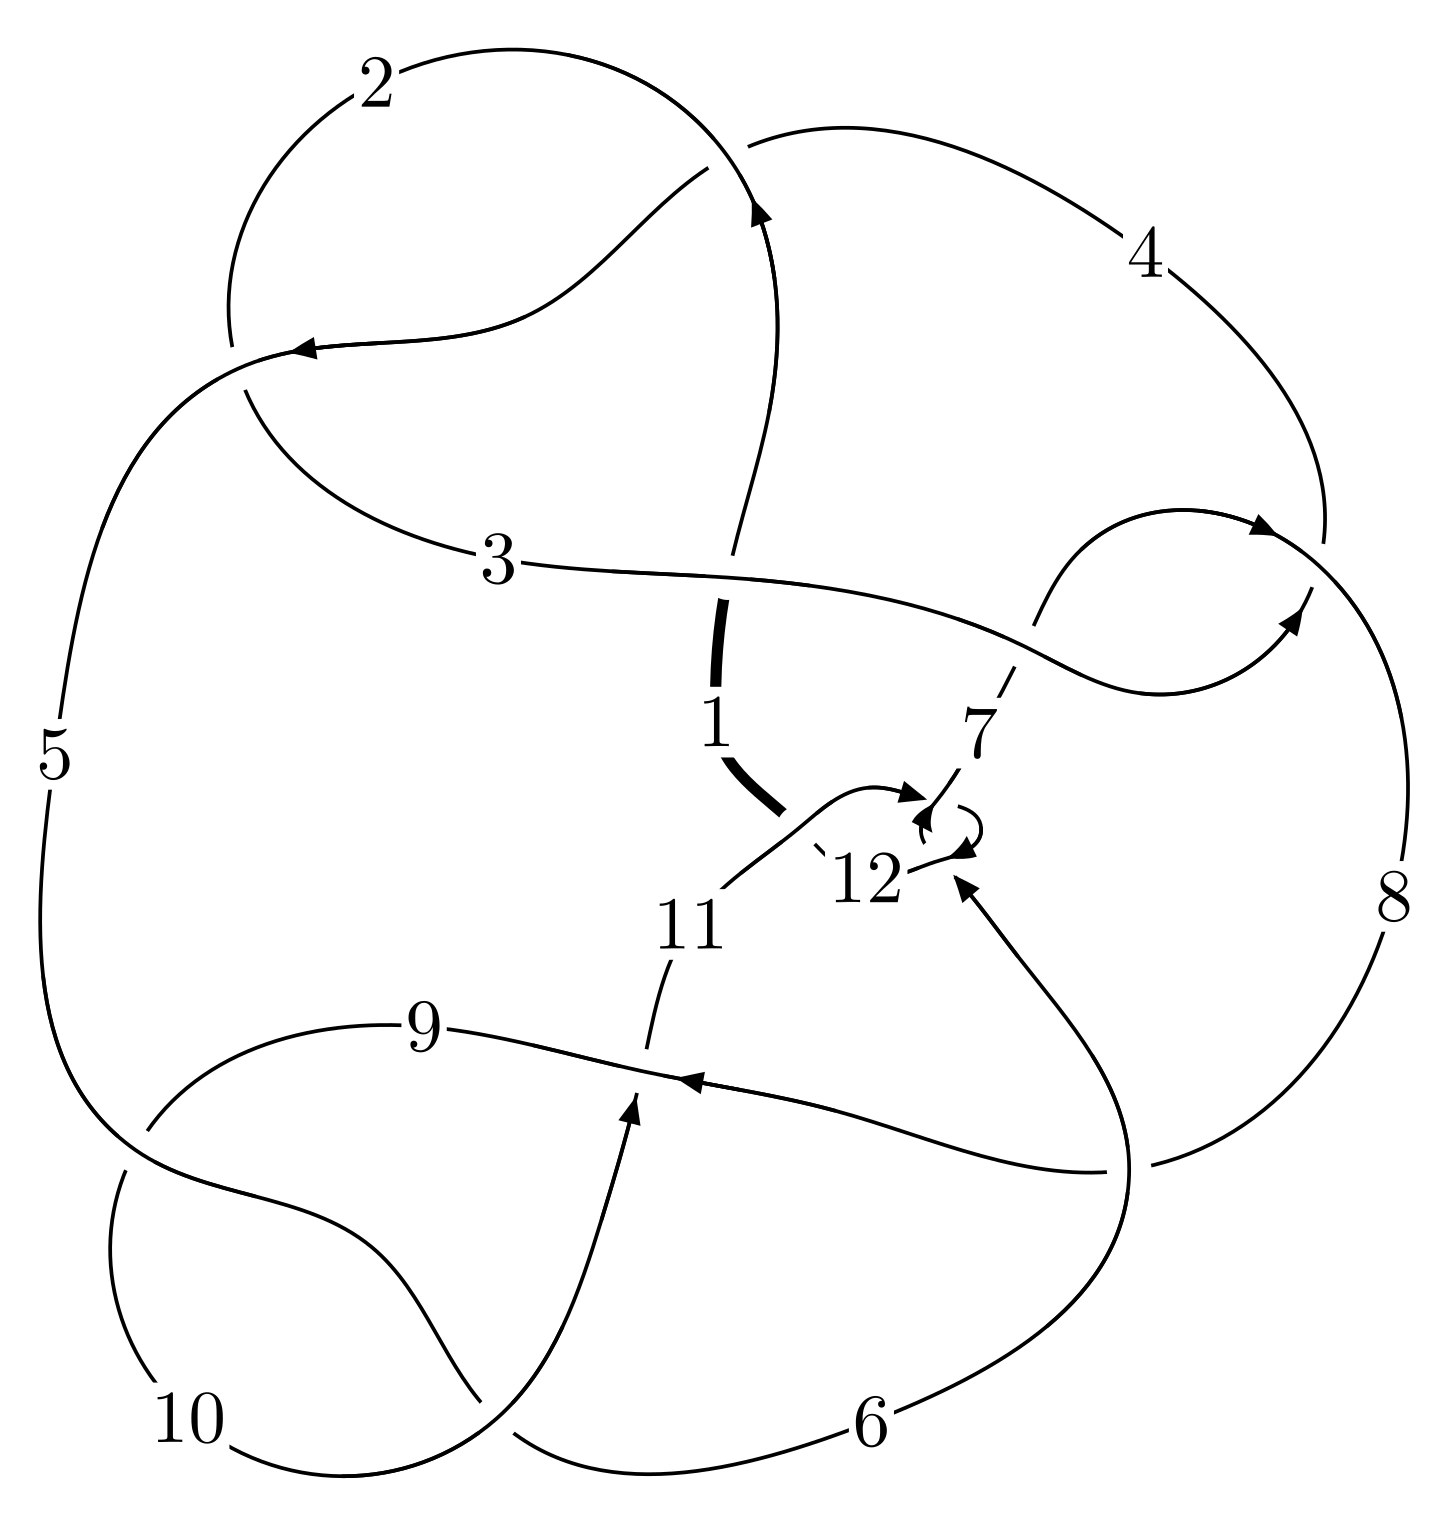
\includegraphics[width=112pt]{../../../GIT/diagram.site/Diagrams/png/2271_12n_0182.png}\\
\ \ \ A knot diagram\footnotemark}&
\allowdisplaybreaks
\textbf{Linearized knot diagam} \\
\cline{2-2}
 &
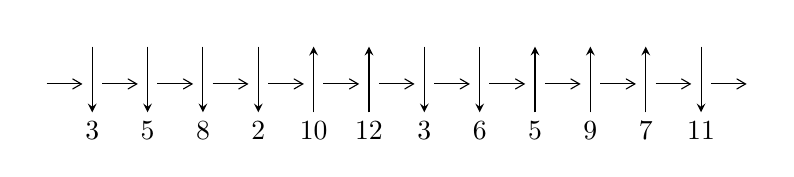
\begin{tikzpicture}[x=20pt, y=17pt]
	% nodes
	\node (C0) at (0, 0) {};
	\node (C1) at (1, 0) {};
	\node (C1U) at (1, +1) {};
	\node (C1D) at (1, -1) {3};

	\node (C2) at (2, 0) {};
	\node (C2U) at (2, +1) {};
	\node (C2D) at (2, -1) {5};

	\node (C3) at (3, 0) {};
	\node (C3U) at (3, +1) {};
	\node (C3D) at (3, -1) {8};

	\node (C4) at (4, 0) {};
	\node (C4U) at (4, +1) {};
	\node (C4D) at (4, -1) {2};

	\node (C5) at (5, 0) {};
	\node (C5U) at (5, +1) {};
	\node (C5D) at (5, -1) {10};

	\node (C6) at (6, 0) {};
	\node (C6U) at (6, +1) {};
	\node (C6D) at (6, -1) {12};

	\node (C7) at (7, 0) {};
	\node (C7U) at (7, +1) {};
	\node (C7D) at (7, -1) {3};

	\node (C8) at (8, 0) {};
	\node (C8U) at (8, +1) {};
	\node (C8D) at (8, -1) {6};

	\node (C9) at (9, 0) {};
	\node (C9U) at (9, +1) {};
	\node (C9D) at (9, -1) {5};

	\node (C10) at (10, 0) {};
	\node (C10U) at (10, +1) {};
	\node (C10D) at (10, -1) {9};

	\node (C11) at (11, 0) {};
	\node (C11U) at (11, +1) {};
	\node (C11D) at (11, -1) {7};

	\node (C12) at (12, 0) {};
	\node (C12U) at (12, +1) {};
	\node (C12D) at (12, -1) {11};
	\node (C13) at (13, 0) {};

	% arrows
	\draw[->,>={angle 60}]
	(C0) edge (C1) (C1) edge (C2) (C2) edge (C3) (C3) edge (C4) (C4) edge (C5) (C5) edge (C6) (C6) edge (C7) (C7) edge (C8) (C8) edge (C9) (C9) edge (C10) (C10) edge (C11) (C11) edge (C12) (C12) edge (C13) ;	\draw[->,>=stealth]
	(C1U) edge (C1D) (C2U) edge (C2D) (C3U) edge (C3D) (C4U) edge (C4D) (C5D) edge (C5U) (C6D) edge (C6U) (C7U) edge (C7D) (C8U) edge (C8D) (C9D) edge (C9U) (C10D) edge (C10U) (C11D) edge (C11U) (C12U) edge (C12D) ;
	\end{tikzpicture} \\
\hhline{~~} \\& 
\textbf{Solving Sequence} \\ \cline{2-2} 
 &
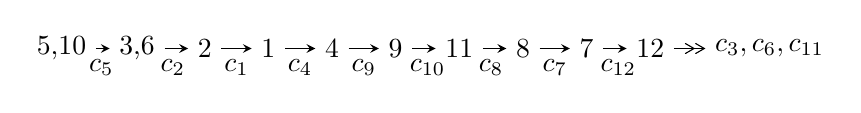
\begin{tikzpicture}[x=23pt, y=7pt]
	% node
	\node (A0) at (-1/8, 0) {5,10};
	\node (A1) at (17/16, 0) {3,6};
	\node (A2) at (17/8, 0) {2};
	\node (A3) at (25/8, 0) {1};
	\node (A4) at (33/8, 0) {4};
	\node (A5) at (41/8, 0) {9};
	\node (A6) at (49/8, 0) {11};
	\node (A7) at (57/8, 0) {8};
	\node (A8) at (65/8, 0) {7};
	\node (A9) at (73/8, 0) {12};
	\node (C1) at (1/2, -1) {$c_{5}$};
	\node (C2) at (13/8, -1) {$c_{2}$};
	\node (C3) at (21/8, -1) {$c_{1}$};
	\node (C4) at (29/8, -1) {$c_{4}$};
	\node (C5) at (37/8, -1) {$c_{9}$};
	\node (C6) at (45/8, -1) {$c_{10}$};
	\node (C7) at (53/8, -1) {$c_{8}$};
	\node (C8) at (61/8, -1) {$c_{7}$};
	\node (C9) at (69/8, -1) {$c_{12}$};
	\node (A10) at (11, 0) {$c_{3},c_{6},c_{11}$};

	% edge
	\draw[->,>=stealth]	
	(A0) edge (A1) (A1) edge (A2) (A2) edge (A3) (A3) edge (A4) (A4) edge (A5) (A5) edge (A6) (A6) edge (A7) (A7) edge (A8) (A8) edge (A9) ;
	\draw[->>,>={angle 60}]	
	(A9) edge (A10);
\end{tikzpicture} \\ 

\end{tabular} \\

\footnotetext{
The image of knot diagram is generated by the software ``\textbf{Draw programme}" developed by Andrew Bartholomew(\url{http://www.layer8.co.uk/maths/draw/index.htm\#Running-draw}), where we modified some parts for our purpose(\url{https://github.com/CATsTAILs/LinksPainter}).
}\phantom \\ \newline 
\centering \textbf{Ideals for irreducible components\footnotemark of $X_{\text{par}}$} 
 
\begin{align*}
I^u_{1}&=\langle 
-1.36510\times10^{17} u^{43}+9.54484\times10^{15} u^{42}+\cdots+1.53293\times10^{18} b+1.33198\times10^{18},\\
\phantom{I^u_{1}}&\phantom{= \langle  }-1.62174\times10^{18} u^{43}+1.01186\times10^{18} u^{42}+\cdots+1.53293\times10^{18} a-2.65681\times10^{18},\;u^{44}-2 u^{43}+\cdots- u-1\rangle \\
I^u_{2}&=\langle 
b+1,\;-2 u^8+u^7+5 u^6-3 u^5-4 u^4+3 u^3-2 u^2+a+2,\;u^9- u^8-2 u^7+3 u^6+u^5-3 u^4+2 u^3- u+1\rangle \\
\\
\end{align*}
\raggedright * 2 irreducible components of $\dim_{\mathbb{C}}=0$, with total 53 representations.\\
\footnotetext{All coefficients of polynomials are rational numbers. But the coefficients are sometimes approximated in decimal forms when there is not enough margin.}
\newpage
\renewcommand{\arraystretch}{1}
\centering \section*{I. $I^u_{1}= \langle -1.37\times10^{17} u^{43}+9.54\times10^{15} u^{42}+\cdots+1.53\times10^{18} b+1.33\times10^{18},\;-1.62\times10^{18} u^{43}+1.01\times10^{18} u^{42}+\cdots+1.53\times10^{18} a-2.66\times10^{18},\;u^{44}-2 u^{43}+\cdots- u-1 \rangle$}
\flushleft \textbf{(i) Arc colorings}\\
\begin{tabular}{m{7pt} m{180pt} m{7pt} m{180pt} }
\flushright $a_{5}=$&$\begin{pmatrix}1\\0\end{pmatrix}$ \\
\flushright $a_{10}=$&$\begin{pmatrix}0\\u\end{pmatrix}$ \\
\flushright $a_{3}=$&$\begin{pmatrix}1.05794 u^{43}-0.660080 u^{42}+\cdots-1.09633 u+1.73316\\0.0890516 u^{43}-0.00622654 u^{42}+\cdots-0.0813299 u-0.868912\end{pmatrix}$ \\
\flushright $a_{6}=$&$\begin{pmatrix}1\\- u^2\end{pmatrix}$ \\
\flushright $a_{2}=$&$\begin{pmatrix}1.14699 u^{43}-0.666307 u^{42}+\cdots-1.17766 u+0.864250\\0.0890516 u^{43}-0.00622654 u^{42}+\cdots-0.0813299 u-0.868912\end{pmatrix}$ \\
\flushright $a_{1}=$&$\begin{pmatrix}0.108274 u^{43}-0.166759 u^{42}+\cdots-0.652412 u-1.28055\\0.0893388 u^{43}-0.0640460 u^{42}+\cdots+0.0125622 u+0.212283\end{pmatrix}$ \\
\flushright $a_{4}=$&$\begin{pmatrix}1.02965 u^{43}-0.560533 u^{42}+\cdots-0.952635 u+1.81995\\0.0297535 u^{43}+0.00665588 u^{42}+\cdots-0.112208 u-0.958338\end{pmatrix}$ \\
\flushright $a_{9}=$&$\begin{pmatrix}- u\\u\end{pmatrix}$ \\
\flushright $a_{11}=$&$\begin{pmatrix}u^3\\- u^3+u\end{pmatrix}$ \\
\flushright $a_{8}=$&$\begin{pmatrix}- u^3\\u^5- u^3+u\end{pmatrix}$ \\
\flushright $a_{7}=$&$\begin{pmatrix}-0.763419 u^{43}+1.17680 u^{42}+\cdots+2.97987 u-0.290205\\0.246436 u^{43}-0.344490 u^{42}+\cdots-0.623825 u+0.0577269\end{pmatrix}$ \\
\flushright $a_{12}=$&$\begin{pmatrix}-0.143931 u^{43}+0.0553767 u^{42}+\cdots-0.710282 u-1.19853\\0.201658 u^{43}+0.0756056 u^{42}+\cdots+0.749462 u+0.516983\end{pmatrix}$\\&\end{tabular}
\flushleft \textbf{(ii) Obstruction class $= -1$}\\~\\
\flushleft \textbf{(iii) Cusp Shapes $= -\frac{1914830631575013385}{510976393730080697} u^{43}+\frac{344553853487150851}{510976393730080697} u^{42}+\cdots+\frac{143617252098136043}{510976393730080697} u-\frac{6332818336569097832}{510976393730080697}$}\\~\\
\newpage\renewcommand{\arraystretch}{1}
\flushleft \textbf{(iv) u-Polynomials at the component}\newline \\
\begin{tabular}{m{50pt}|m{274pt}}
Crossings & \hspace{64pt}u-Polynomials at each crossing \\
\hline $$\begin{aligned}c_{1}\end{aligned}$$&$\begin{aligned}
&u^{44}+58 u^{43}+\cdots+579 u+1
\end{aligned}$\\
\hline $$\begin{aligned}c_{2},c_{4}\end{aligned}$$&$\begin{aligned}
&u^{44}-10 u^{43}+\cdots-39 u-1
\end{aligned}$\\
\hline $$\begin{aligned}c_{3},c_{7}\end{aligned}$$&$\begin{aligned}
&u^{44}- u^{43}+\cdots+8192 u+512
\end{aligned}$\\
\hline $$\begin{aligned}c_{5},c_{9}\end{aligned}$$&$\begin{aligned}
&u^{44}-2 u^{43}+\cdots- u-1
\end{aligned}$\\
\hline $$\begin{aligned}c_{6},c_{11}\end{aligned}$$&$\begin{aligned}
&u^{44}-2 u^{43}+\cdots- u-1
\end{aligned}$\\
\hline $$\begin{aligned}c_{8}\end{aligned}$$&$\begin{aligned}
&u^{44}-6 u^{43}+\cdots+537 u+117
\end{aligned}$\\
\hline $$\begin{aligned}c_{10}\end{aligned}$$&$\begin{aligned}
&u^{44}-18 u^{43}+\cdots-15 u+1
\end{aligned}$\\
\hline $$\begin{aligned}c_{12}\end{aligned}$$&$\begin{aligned}
&u^{44}+30 u^{43}+\cdots-15 u+1
\end{aligned}$\\
\hline
\end{tabular}\\~\\
\newpage\renewcommand{\arraystretch}{1}
\flushleft \textbf{(v) Riley Polynomials at the component}\newline \\
\begin{tabular}{m{50pt}|m{274pt}}
Crossings & \hspace{64pt}Riley Polynomials at each crossing \\
\hline $$\begin{aligned}c_{1}\end{aligned}$$&$\begin{aligned}
&y^{44}-134 y^{43}+\cdots+635013 y+1
\end{aligned}$\\
\hline $$\begin{aligned}c_{2},c_{4}\end{aligned}$$&$\begin{aligned}
&y^{44}-58 y^{43}+\cdots-579 y+1
\end{aligned}$\\
\hline $$\begin{aligned}c_{3},c_{7}\end{aligned}$$&$\begin{aligned}
&y^{44}-57 y^{43}+\cdots-14417920 y+262144
\end{aligned}$\\
\hline $$\begin{aligned}c_{5},c_{9}\end{aligned}$$&$\begin{aligned}
&y^{44}-18 y^{43}+\cdots-15 y+1
\end{aligned}$\\
\hline $$\begin{aligned}c_{6},c_{11}\end{aligned}$$&$\begin{aligned}
&y^{44}+30 y^{43}+\cdots-15 y+1
\end{aligned}$\\
\hline $$\begin{aligned}c_{8}\end{aligned}$$&$\begin{aligned}
&y^{44}-18 y^{43}+\cdots-749115 y+13689
\end{aligned}$\\
\hline $$\begin{aligned}c_{10}\end{aligned}$$&$\begin{aligned}
&y^{44}+18 y^{43}+\cdots-103 y+1
\end{aligned}$\\
\hline $$\begin{aligned}c_{12}\end{aligned}$$&$\begin{aligned}
&y^{44}-30 y^{43}+\cdots-303 y+1
\end{aligned}$\\
\hline
\end{tabular}\\~\\
\newpage\flushleft \textbf{(vi) Complex Volumes and Cusp Shapes}
$$\begin{array}{c|c|c}  
\text{Solutions to }I^u_{1}& \I (\text{vol} + \sqrt{-1}CS) & \text{Cusp shape}\\
 \hline 
\begin{aligned}
u &= \phantom{-}0.688110 + 0.685606 I \\
a &= \phantom{-}0.863564 + 0.136667 I \\
b &= -1.10774 - 1.23190 I\end{aligned}
 & -5.98385 - 2.15414 I & -9.20742 + 2.18421 I \\ \hline\begin{aligned}
u &= \phantom{-}0.688110 - 0.685606 I \\
a &= \phantom{-}0.863564 - 0.136667 I \\
b &= -1.10774 + 1.23190 I\end{aligned}
 & -5.98385 + 2.15414 I & -9.20742 - 2.18421 I \\ \hline\begin{aligned}
u &= \phantom{-}0.845683 + 0.592317 I \\
a &= -1.25164 - 1.23315 I \\
b &= -1.243990 + 0.046469 I\end{aligned}
 & -3.00115 + 2.34547 I & \phantom{-}0.61315 - 3.20636 I \\ \hline\begin{aligned}
u &= \phantom{-}0.845683 - 0.592317 I \\
a &= -1.25164 + 1.23315 I \\
b &= -1.243990 - 0.046469 I\end{aligned}
 & -3.00115 - 2.34547 I & \phantom{-}0.61315 + 3.20636 I \\ \hline\begin{aligned}
u &= \phantom{-}0.905356 + 0.530754 I \\
a &= \phantom{-}1.20385 - 5.40977 I \\
b &= -0.922690 + 0.021453 I\end{aligned}
 & -3.18610 + 2.04679 I & -26.8865 + 3.7587 I \\ \hline\begin{aligned}
u &= \phantom{-}0.905356 - 0.530754 I \\
a &= \phantom{-}1.20385 + 5.40977 I \\
b &= -0.922690 - 0.021453 I\end{aligned}
 & -3.18610 - 2.04679 I & -26.8865 - 3.7587 I \\ \hline\begin{aligned}
u &= \phantom{-}0.515365 + 0.921554 I \\
a &= \phantom{-}0.0523760 - 0.1117110 I \\
b &= \phantom{-}1.80210 + 0.36838 I\end{aligned}
 & -15.2823 - 8.3356 I & -7.68501 + 3.11371 I \\ \hline\begin{aligned}
u &= \phantom{-}0.515365 - 0.921554 I \\
a &= \phantom{-}0.0523760 + 0.1117110 I \\
b &= \phantom{-}1.80210 - 0.36838 I\end{aligned}
 & -15.2823 + 8.3356 I & -7.68501 - 3.11371 I \\ \hline\begin{aligned}
u &= \phantom{-}0.497628 + 0.931746 I \\
a &= \phantom{-}0.0477482 + 0.1144550 I \\
b &= \phantom{-}1.79749 - 0.07891 I\end{aligned}
 & -15.1569 + 3.5164 I & -7.98502 - 2.64030 I \\ \hline\begin{aligned}
u &= \phantom{-}0.497628 - 0.931746 I \\
a &= \phantom{-}0.0477482 - 0.1144550 I \\
b &= \phantom{-}1.79749 + 0.07891 I\end{aligned}
 & -15.1569 - 3.5164 I & -7.98502 + 2.64030 I\\
 \hline 
 \end{array}$$\newpage$$\begin{array}{c|c|c}  
\text{Solutions to }I^u_{1}& \I (\text{vol} + \sqrt{-1}CS) & \text{Cusp shape}\\
 \hline 
\begin{aligned}
u &= -0.804579 + 0.489610 I \\
a &= \phantom{-}1.071560 - 0.142770 I \\
b &= -0.0319136 - 0.0206061 I\end{aligned}
 & -1.74326 - 2.05593 I & -4.38426 + 3.93247 I \\ \hline\begin{aligned}
u &= -0.804579 - 0.489610 I \\
a &= \phantom{-}1.071560 + 0.142770 I \\
b &= -0.0319136 + 0.0206061 I\end{aligned}
 & -1.74326 + 2.05593 I & -4.38426 - 3.93247 I \\ \hline\begin{aligned}
u &= -0.511016 + 0.933628 I \\
a &= \phantom{-}0.0888703 - 0.0020707 I \\
b &= \phantom{-}1.71985 - 0.15282 I\end{aligned}
 & -10.83690 + 2.46216 I & -5.51655 - 0.44407 I \\ \hline\begin{aligned}
u &= -0.511016 - 0.933628 I \\
a &= \phantom{-}0.0888703 + 0.0020707 I \\
b &= \phantom{-}1.71985 + 0.15282 I\end{aligned}
 & -10.83690 - 2.46216 I & -5.51655 + 0.44407 I \\ \hline\begin{aligned}
u &= -0.849836 + 0.684332 I \\
a &= \phantom{-}0.27393 + 1.58284 I \\
b &= -2.08374 - 0.15007 I\end{aligned}
 & -7.96382 - 2.63414 I & -10.69768 + 3.24229 I \\ \hline\begin{aligned}
u &= -0.849836 - 0.684332 I \\
a &= \phantom{-}0.27393 - 1.58284 I \\
b &= -2.08374 + 0.15007 I\end{aligned}
 & -7.96382 + 2.63414 I & -10.69768 - 3.24229 I \\ \hline\begin{aligned}
u &= \phantom{-}0.880721 + 0.195510 I \\
a &= \phantom{-}0.851230 + 0.816240 I \\
b &= \phantom{-}0.027650 - 0.386682 I\end{aligned}
 & \phantom{-}1.49461 + 0.44791 I & \phantom{-}5.81228 - 0.84575 I \\ \hline\begin{aligned}
u &= \phantom{-}0.880721 - 0.195510 I \\
a &= \phantom{-}0.851230 - 0.816240 I \\
b &= \phantom{-}0.027650 + 0.386682 I\end{aligned}
 & \phantom{-}1.49461 - 0.44791 I & \phantom{-}5.81228 + 0.84575 I \\ \hline\begin{aligned}
u &= -0.698557 + 0.569479 I \\
a &= \phantom{-}0.474798 - 0.585716 I \\
b &= -0.826219 + 0.509582 I\end{aligned}
 & -1.84063 - 0.16201 I & -3.33593 + 0.20561 I \\ \hline\begin{aligned}
u &= -0.698557 - 0.569479 I \\
a &= \phantom{-}0.474798 + 0.585716 I \\
b &= -0.826219 - 0.509582 I\end{aligned}
 & -1.84063 + 0.16201 I & -3.33593 - 0.20561 I\\
 \hline 
 \end{array}$$\newpage$$\begin{array}{c|c|c}  
\text{Solutions to }I^u_{1}& \I (\text{vol} + \sqrt{-1}CS) & \text{Cusp shape}\\
 \hline 
\begin{aligned}
u &= -0.960365 + 0.600329 I \\
a &= -0.22638 + 1.69062 I \\
b &= -0.608152 - 0.737629 I\end{aligned}
 & -1.02255 - 4.55319 I & -0.74748 + 6.17596 I \\ \hline\begin{aligned}
u &= -0.960365 - 0.600329 I \\
a &= -0.22638 - 1.69062 I \\
b &= -0.608152 + 0.737629 I\end{aligned}
 & -1.02255 + 4.55319 I & -0.74748 - 6.17596 I \\ \hline\begin{aligned}
u &= -0.860051 + 0.047625 I \\
a &= \phantom{-}1.74194 + 1.29974 I \\
b &= -0.364953 - 0.686094 I\end{aligned}
 & -1.23921 - 2.55790 I & -0.72063 + 3.92676 I \\ \hline\begin{aligned}
u &= -0.860051 - 0.047625 I \\
a &= \phantom{-}1.74194 - 1.29974 I \\
b &= -0.364953 + 0.686094 I\end{aligned}
 & -1.23921 + 2.55790 I & -0.72063 - 3.92676 I \\ \hline\begin{aligned}
u &= \phantom{-}0.970487 + 0.654541 I \\
a &= -0.73443 - 1.96174 I \\
b &= -0.86872 + 1.43316 I\end{aligned}
 & -5.13822 + 7.34601 I & -6.99400 - 7.81515 I \\ \hline\begin{aligned}
u &= \phantom{-}0.970487 - 0.654541 I \\
a &= -0.73443 + 1.96174 I \\
b &= -0.86872 - 1.43316 I\end{aligned}
 & -5.13822 - 7.34601 I & -6.99400 + 7.81515 I \\ \hline\begin{aligned}
u &= \phantom{-}1.132370 + 0.387785 I \\
a &= -0.128368 + 0.373910 I \\
b &= \phantom{-}0.558289 + 0.000722 I\end{aligned}
 & \phantom{-}3.49180 + 1.33135 I & \phantom{-}7.33904 - 0.67803 I \\ \hline\begin{aligned}
u &= \phantom{-}1.132370 - 0.387785 I \\
a &= -0.128368 - 0.373910 I \\
b &= \phantom{-}0.558289 - 0.000722 I\end{aligned}
 & \phantom{-}3.49180 - 1.33135 I & \phantom{-}7.33904 + 0.67803 I \\ \hline\begin{aligned}
u &= -1.137390 + 0.514032 I \\
a &= -0.404883 - 0.128194 I \\
b &= \phantom{-}0.649155 - 0.317441 I\end{aligned}
 & \phantom{-}2.59233 - 6.57074 I & \phantom{-}3.54533 + 3.81879 I \\ \hline\begin{aligned}
u &= -1.137390 - 0.514032 I \\
a &= -0.404883 + 0.128194 I \\
b &= \phantom{-}0.649155 + 0.317441 I\end{aligned}
 & \phantom{-}2.59233 + 6.57074 I & \phantom{-}3.54533 - 3.81879 I\\
 \hline 
 \end{array}$$\newpage$$\begin{array}{c|c|c}  
\text{Solutions to }I^u_{1}& \I (\text{vol} + \sqrt{-1}CS) & \text{Cusp shape}\\
 \hline 
\begin{aligned}
u &= -1.270670 + 0.015648 I \\
a &= -1.99358 - 0.44608 I \\
b &= \phantom{-}1.65558 + 0.23166 I\end{aligned}
 & -8.56328 - 6.02412 I & -2.00000 + 3.26167 I \\ \hline\begin{aligned}
u &= -1.270670 - 0.015648 I \\
a &= -1.99358 + 0.44608 I \\
b &= \phantom{-}1.65558 - 0.23166 I\end{aligned}
 & -8.56328 + 6.02412 I & -2.00000 - 3.26167 I \\ \hline\begin{aligned}
u &= \phantom{-}1.28468\phantom{ +0.000000I} \\
a &= -1.81405\phantom{ +0.000000I} \\
b &= \phantom{-}1.56686\phantom{ +0.000000I}\end{aligned}
 & -4.09522\phantom{ +0.000000I} & -1.39870\phantom{ +0.000000I} \\ \hline\begin{aligned}
u &= \phantom{-}1.121640 + 0.694109 I \\
a &= -0.38211 + 2.16430 I \\
b &= \phantom{-}1.76719 - 0.45741 I\end{aligned}
 & -13.4269 + 14.2723 I & \phantom{-0.000000 } 0 \\ \hline\begin{aligned}
u &= \phantom{-}1.121640 - 0.694109 I \\
a &= -0.38211 - 2.16430 I \\
b &= \phantom{-}1.76719 + 0.45741 I\end{aligned}
 & -13.4269 - 14.2723 I & \phantom{-0.000000 } 0 \\ \hline\begin{aligned}
u &= -0.194814 + 0.648377 I \\
a &= \phantom{-}0.686468 - 0.152693 I \\
b &= \phantom{-}0.408342 + 0.262891 I\end{aligned}
 & -0.02630 + 2.06519 I & \phantom{-}0.09253 - 2.36039 I \\ \hline\begin{aligned}
u &= -0.194814 - 0.648377 I \\
a &= \phantom{-}0.686468 + 0.152693 I \\
b &= \phantom{-}0.408342 - 0.262891 I\end{aligned}
 & -0.02630 - 2.06519 I & \phantom{-}0.09253 + 2.36039 I \\ \hline\begin{aligned}
u &= -1.128940 + 0.699014 I \\
a &= -0.50088 - 1.83474 I \\
b &= \phantom{-}1.68302 + 0.25609 I\end{aligned}
 & -8.94545 - 8.44958 I & \phantom{-0.000000 } 0 \\ \hline\begin{aligned}
u &= -1.128940 - 0.699014 I \\
a &= -0.50088 + 1.83474 I \\
b &= \phantom{-}1.68302 - 0.25609 I\end{aligned}
 & -8.94545 + 8.44958 I & \phantom{-0.000000 } 0 \\ \hline\begin{aligned}
u &= \phantom{-}1.136310 + 0.692427 I \\
a &= -0.83675 + 1.65755 I \\
b &= \phantom{-}1.75390 - 0.02647 I\end{aligned}
 & -13.20280 + 2.44542 I & \phantom{-0.000000 } 0\\
 \hline 
 \end{array}$$\newpage$$\begin{array}{c|c|c}  
\text{Solutions to }I^u_{1}& \I (\text{vol} + \sqrt{-1}CS) & \text{Cusp shape}\\
 \hline 
\begin{aligned}
u &= \phantom{-}1.136310 - 0.692427 I \\
a &= -0.83675 - 1.65755 I \\
b &= \phantom{-}1.75390 + 0.02647 I\end{aligned}
 & -13.20280 - 2.44542 I & \phantom{-0.000000 } 0 \\ \hline\begin{aligned}
u &= \phantom{-}0.228003 + 0.393046 I \\
a &= \phantom{-}2.05111 - 0.21934 I \\
b &= -1.129040 + 0.431943 I\end{aligned}
 & -4.33669 + 1.37214 I & -7.87004 - 0.50855 I \\ \hline\begin{aligned}
u &= \phantom{-}0.228003 - 0.393046 I \\
a &= \phantom{-}2.05111 + 0.21934 I \\
b &= -1.129040 - 0.431943 I\end{aligned}
 & -4.33669 - 1.37214 I & -7.87004 + 0.50855 I \\ \hline\begin{aligned}
u &= -0.295609\phantom{ +0.000000I} \\
a &= \phantom{-}1.91719\phantom{ +0.000000I} \\
b &= -0.837652\phantom{ +0.000000I}\end{aligned}
 & -1.20532\phantom{ +0.000000I} & -9.09590\phantom{ +0.000000I}\\
 \hline 
 \end{array}$$\newpage\newpage\renewcommand{\arraystretch}{1}
\centering \section*{II. $I^u_{2}= \langle b+1,\;-2 u^8+u^7+\cdots+a+2,\;u^9- u^8-2 u^7+3 u^6+u^5-3 u^4+2 u^3- u+1 \rangle$}
\flushleft \textbf{(i) Arc colorings}\\
\begin{tabular}{m{7pt} m{180pt} m{7pt} m{180pt} }
\flushright $a_{5}=$&$\begin{pmatrix}1\\0\end{pmatrix}$ \\
\flushright $a_{10}=$&$\begin{pmatrix}0\\u\end{pmatrix}$ \\
\flushright $a_{3}=$&$\begin{pmatrix}2 u^8- u^7-5 u^6+3 u^5+4 u^4-3 u^3+2 u^2-2\\-1\end{pmatrix}$ \\
\flushright $a_{6}=$&$\begin{pmatrix}1\\- u^2\end{pmatrix}$ \\
\flushright $a_{2}=$&$\begin{pmatrix}2 u^8- u^7-5 u^6+3 u^5+4 u^4-3 u^3+2 u^2-3\\-1\end{pmatrix}$ \\
\flushright $a_{1}=$&$\begin{pmatrix}-1\\0\end{pmatrix}$ \\
\flushright $a_{4}=$&$\begin{pmatrix}2 u^8- u^7-5 u^6+3 u^5+4 u^4-3 u^3+2 u^2-2\\-1\end{pmatrix}$ \\
\flushright $a_{9}=$&$\begin{pmatrix}- u\\u\end{pmatrix}$ \\
\flushright $a_{11}=$&$\begin{pmatrix}u^3\\- u^3+u\end{pmatrix}$ \\
\flushright $a_{8}=$&$\begin{pmatrix}- u^3\\u^5- u^3+u\end{pmatrix}$ \\
\flushright $a_{7}=$&$\begin{pmatrix}- u^3\\u^5- u^3+u\end{pmatrix}$ \\
\flushright $a_{12}=$&$\begin{pmatrix}- u^6+u^4-1\\u^6-2 u^4+u^2\end{pmatrix}$\\&\end{tabular}
\flushleft \textbf{(ii) Obstruction class $= 1$}\\~\\
\flushleft \textbf{(iii) Cusp Shapes $= 6 u^8-3 u^7-10 u^6+8 u^5+2 u^4-8 u^3+12 u^2-6$}\\~\\
\newpage\renewcommand{\arraystretch}{1}
\flushleft \textbf{(iv) u-Polynomials at the component}\newline \\
\begin{tabular}{m{50pt}|m{274pt}}
Crossings & \hspace{64pt}u-Polynomials at each crossing \\
\hline $$\begin{aligned}c_{1},c_{2}\end{aligned}$$&$\begin{aligned}
&(u-1)^9
\end{aligned}$\\
\hline $$\begin{aligned}c_{3},c_{7}\end{aligned}$$&$\begin{aligned}
&u^9
\end{aligned}$\\
\hline $$\begin{aligned}c_{4}\end{aligned}$$&$\begin{aligned}
&(u+1)^9
\end{aligned}$\\
\hline $$\begin{aligned}c_{5}\end{aligned}$$&$\begin{aligned}
&u^9- u^8-2 u^7+3 u^6+u^5-3 u^4+2 u^3- u+1
\end{aligned}$\\
\hline $$\begin{aligned}c_{6}\end{aligned}$$&$\begin{aligned}
&u^9- u^8+2 u^7- u^6+3 u^5- u^4+2 u^3+u+1
\end{aligned}$\\
\hline $$\begin{aligned}c_{8},c_{12}\end{aligned}$$&$\begin{aligned}
&u^9+3 u^8+8 u^7+13 u^6+17 u^5+17 u^4+12 u^3+6 u^2+u-1
\end{aligned}$\\
\hline $$\begin{aligned}c_{9}\end{aligned}$$&$\begin{aligned}
&u^9+u^8-2 u^7-3 u^6+u^5+3 u^4+2 u^3- u-1
\end{aligned}$\\
\hline $$\begin{aligned}c_{10}\end{aligned}$$&$\begin{aligned}
&u^9-5 u^8+12 u^7-15 u^6+9 u^5+u^4-4 u^3+2 u^2+u-1
\end{aligned}$\\
\hline $$\begin{aligned}c_{11}\end{aligned}$$&$\begin{aligned}
&u^9+u^8+2 u^7+u^6+3 u^5+u^4+2 u^3+u-1
\end{aligned}$\\
\hline
\end{tabular}\\~\\
\newpage\renewcommand{\arraystretch}{1}
\flushleft \textbf{(v) Riley Polynomials at the component}\newline \\
\begin{tabular}{m{50pt}|m{274pt}}
Crossings & \hspace{64pt}Riley Polynomials at each crossing \\
\hline $$\begin{aligned}c_{1},c_{2},c_{4}\end{aligned}$$&$\begin{aligned}
&(y-1)^9
\end{aligned}$\\
\hline $$\begin{aligned}c_{3},c_{7}\end{aligned}$$&$\begin{aligned}
&y^9
\end{aligned}$\\
\hline $$\begin{aligned}c_{5},c_{9}\end{aligned}$$&$\begin{aligned}
&y^9-5 y^8+12 y^7-15 y^6+9 y^5+y^4-4 y^3+2 y^2+y-1
\end{aligned}$\\
\hline $$\begin{aligned}c_{6},c_{11}\end{aligned}$$&$\begin{aligned}
&y^9+3 y^8+8 y^7+13 y^6+17 y^5+17 y^4+12 y^3+6 y^2+y-1
\end{aligned}$\\
\hline $$\begin{aligned}c_{8},c_{12}\end{aligned}$$&$\begin{aligned}
&y^9+7 y^8+20 y^7+25 y^6+5 y^5-15 y^4+22 y^2+13 y-1
\end{aligned}$\\
\hline $$\begin{aligned}c_{10}\end{aligned}$$&$\begin{aligned}
&y^9- y^8+12 y^7-7 y^6+37 y^5+y^4-10 y^2+5 y-1
\end{aligned}$\\
\hline
\end{tabular}\\~\\
\newpage\flushleft \textbf{(vi) Complex Volumes and Cusp Shapes}
$$\begin{array}{c|c|c}  
\text{Solutions to }I^u_{2}& \I (\text{vol} + \sqrt{-1}CS) & \text{Cusp shape}\\
 \hline 
\begin{aligned}
u &= \phantom{-}0.772920 + 0.510351 I \\
a &= -1.67861 + 2.31573 I \\
b &= -1.00000\phantom{ +0.000000I}\end{aligned}
 & -3.42837 + 2.09337 I & -0.35753 + 5.88316 I \\ \hline\begin{aligned}
u &= \phantom{-}0.772920 - 0.510351 I \\
a &= -1.67861 - 2.31573 I \\
b &= -1.00000\phantom{ +0.000000I}\end{aligned}
 & -3.42837 - 2.09337 I & -0.35753 - 5.88316 I \\ \hline\begin{aligned}
u &= -0.825933\phantom{ +0.000000I} \\
a &= \phantom{-}0.871015\phantom{ +0.000000I} \\
b &= -1.00000\phantom{ +0.000000I}\end{aligned}
 & -0.446489\phantom{ +0.000000I} & \phantom{-}3.46070\phantom{ +0.000000I} \\ \hline\begin{aligned}
u &= -1.173910 + 0.391555 I \\
a &= \phantom{-}0.893484 + 0.630694 I \\
b &= -1.00000\phantom{ +0.000000I}\end{aligned}
 & \phantom{-}2.72642 - 1.33617 I & -4.05086 + 0.75351 I \\ \hline\begin{aligned}
u &= -1.173910 - 0.391555 I \\
a &= \phantom{-}0.893484 - 0.630694 I \\
b &= -1.00000\phantom{ +0.000000I}\end{aligned}
 & \phantom{-}2.72642 + 1.33617 I & -4.05086 - 0.75351 I \\ \hline\begin{aligned}
u &= \phantom{-}0.141484 + 0.739668 I \\
a &= -0.309843 + 0.043204 I \\
b &= -1.00000\phantom{ +0.000000I}\end{aligned}
 & -1.02799 - 2.45442 I & -7.24378 + 3.91612 I \\ \hline\begin{aligned}
u &= \phantom{-}0.141484 - 0.739668 I \\
a &= -0.309843 - 0.043204 I \\
b &= -1.00000\phantom{ +0.000000I}\end{aligned}
 & -1.02799 + 2.45442 I & -7.24378 - 3.91612 I \\ \hline\begin{aligned}
u &= \phantom{-}1.172470 + 0.500383 I \\
a &= \phantom{-}0.659464 - 0.874093 I \\
b &= -1.00000\phantom{ +0.000000I}\end{aligned}
 & \phantom{-}1.95319 + 7.08493 I & -4.07818 - 8.89461 I \\ \hline\begin{aligned}
u &= \phantom{-}1.172470 - 0.500383 I \\
a &= \phantom{-}0.659464 + 0.874093 I \\
b &= -1.00000\phantom{ +0.000000I}\end{aligned}
 & \phantom{-}1.95319 - 7.08493 I & -4.07818 + 8.89461 I\\
 \hline 
 \end{array}$$\newpage
\newpage\renewcommand{\arraystretch}{1}
\centering \section*{ III. u-Polynomials}
\begin{tabular}{m{50pt}|m{274pt}}
Crossings & \hspace{64pt}u-Polynomials at each crossing \\
\hline $$\begin{aligned}c_{1}\end{aligned}$$&$\begin{aligned}
&((u-1)^9)(u^{44}+58 u^{43}+\cdots+579 u+1)
\end{aligned}$\\
\hline $$\begin{aligned}c_{2}\end{aligned}$$&$\begin{aligned}
&((u-1)^9)(u^{44}-10 u^{43}+\cdots-39 u-1)
\end{aligned}$\\
\hline $$\begin{aligned}c_{3},c_{7}\end{aligned}$$&$\begin{aligned}
&u^9(u^{44}- u^{43}+\cdots+8192 u+512)
\end{aligned}$\\
\hline $$\begin{aligned}c_{4}\end{aligned}$$&$\begin{aligned}
&((u+1)^9)(u^{44}-10 u^{43}+\cdots-39 u-1)
\end{aligned}$\\
\hline $$\begin{aligned}c_{5}\end{aligned}$$&$\begin{aligned}
&(u^9- u^8+\cdots- u+1)(u^{44}-2 u^{43}+\cdots- u-1)
\end{aligned}$\\
\hline $$\begin{aligned}c_{6}\end{aligned}$$&$\begin{aligned}
&(u^9- u^8+\cdots+u+1)(u^{44}-2 u^{43}+\cdots- u-1)
\end{aligned}$\\
\hline $$\begin{aligned}c_{8}\end{aligned}$$&$\begin{aligned}
&(u^9+3 u^8+8 u^7+13 u^6+17 u^5+17 u^4+12 u^3+6 u^2+u-1)\\
&\cdot(u^{44}-6 u^{43}+\cdots+537 u+117)
\end{aligned}$\\
\hline $$\begin{aligned}c_{9}\end{aligned}$$&$\begin{aligned}
&(u^9+u^8+\cdots- u-1)(u^{44}-2 u^{43}+\cdots- u-1)
\end{aligned}$\\
\hline $$\begin{aligned}c_{10}\end{aligned}$$&$\begin{aligned}
&(u^9-5 u^8+12 u^7-15 u^6+9 u^5+u^4-4 u^3+2 u^2+u-1)\\
&\cdot(u^{44}-18 u^{43}+\cdots-15 u+1)
\end{aligned}$\\
\hline $$\begin{aligned}c_{11}\end{aligned}$$&$\begin{aligned}
&(u^9+u^8+\cdots+u-1)(u^{44}-2 u^{43}+\cdots- u-1)
\end{aligned}$\\
\hline $$\begin{aligned}c_{12}\end{aligned}$$&$\begin{aligned}
&(u^9+3 u^8+8 u^7+13 u^6+17 u^5+17 u^4+12 u^3+6 u^2+u-1)\\
&\cdot(u^{44}+30 u^{43}+\cdots-15 u+1)
\end{aligned}$\\
\hline
\end{tabular}\newpage\renewcommand{\arraystretch}{1}
\centering \section*{ IV. Riley Polynomials}
\begin{tabular}{m{50pt}|m{274pt}}
Crossings & \hspace{64pt}Riley Polynomials at each crossing \\
\hline $$\begin{aligned}c_{1}\end{aligned}$$&$\begin{aligned}
&((y-1)^9)(y^{44}-134 y^{43}+\cdots+635013 y+1)
\end{aligned}$\\
\hline $$\begin{aligned}c_{2},c_{4}\end{aligned}$$&$\begin{aligned}
&((y-1)^9)(y^{44}-58 y^{43}+\cdots-579 y+1)
\end{aligned}$\\
\hline $$\begin{aligned}c_{3},c_{7}\end{aligned}$$&$\begin{aligned}
&y^9(y^{44}-57 y^{43}+\cdots-1.44179\times10^{7} y+262144)
\end{aligned}$\\
\hline $$\begin{aligned}c_{5},c_{9}\end{aligned}$$&$\begin{aligned}
&(y^9-5 y^8+12 y^7-15 y^6+9 y^5+y^4-4 y^3+2 y^2+y-1)\\
&\cdot(y^{44}-18 y^{43}+\cdots-15 y+1)
\end{aligned}$\\
\hline $$\begin{aligned}c_{6},c_{11}\end{aligned}$$&$\begin{aligned}
&(y^9+3 y^8+8 y^7+13 y^6+17 y^5+17 y^4+12 y^3+6 y^2+y-1)\\
&\cdot(y^{44}+30 y^{43}+\cdots-15 y+1)
\end{aligned}$\\
\hline $$\begin{aligned}c_{8}\end{aligned}$$&$\begin{aligned}
&(y^9+7 y^8+20 y^7+25 y^6+5 y^5-15 y^4+22 y^2+13 y-1)\\
&\cdot(y^{44}-18 y^{43}+\cdots-749115 y+13689)
\end{aligned}$\\
\hline $$\begin{aligned}c_{10}\end{aligned}$$&$\begin{aligned}
&(y^9- y^8+12 y^7-7 y^6+37 y^5+y^4-10 y^2+5 y-1)\\
&\cdot(y^{44}+18 y^{43}+\cdots-103 y+1)
\end{aligned}$\\
\hline $$\begin{aligned}c_{12}\end{aligned}$$&$\begin{aligned}
&(y^9+7 y^8+20 y^7+25 y^6+5 y^5-15 y^4+22 y^2+13 y-1)\\
&\cdot(y^{44}-30 y^{43}+\cdots-303 y+1)
\end{aligned}$\\
\hline
\end{tabular}
\vskip 2pc
\end{document}